\chapter{Modelo para o PAPD}
\label{cap:modelo-para-o-papd}

A construção de um modelo de PI para o problema de alocação de professores da UFC-Quixadá demanda o conhecimento de algumas informações relevantes no domínio do problema. Dessa forma, foi feito um levantamento de como é realizada atualmente a alocação na UFC-Quixadá, e chegamos a informações que são importantes para a alocação dos professores e das disciplinas. 

A alocação é feita sobre uma grade de horários semanal. Cada elemento dessa grade representa um horário disponível para alocação ao qual chamamos de \textbf{\textit{slot}}. Um \textit{slot} tem o valor de dois créditos (2 horas), ou seja, uma disciplinas de quatro créditos demanda dois \textit{slots} para ser alocada. Um único dia agrupa seis \textit{slots}, aos quais estão divididos nos três turnos de um dia (manhã, tarde e noite). Um turno de um dia agrupa dois \textit{slots}, o \textit{slot} AB e o \textit{slot} CD do turno. 

Neste trabalho, mapeamos os \textit{slots} para valores inteiros, dessa forma os \textit{slots} da segunda-feira são representados pelos valores: 1, 2, 3, 4, 5 e 6; os da terça-feira: 7, 8, 9, 10, 11 e 12; e assim por diante. A tabela abaixo mostra de forma completa como os \textit{slots} estão organizados na grade de horários.

\begin{figure}[htbp]
	\centering
	\IBGEtab{
		\Caption{\label{figura-1}Tabela de slots}		
    }{
		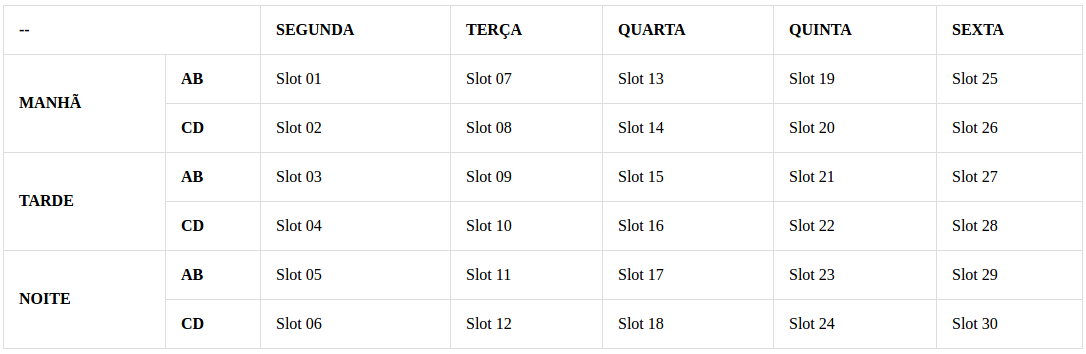
\includegraphics[scale=0.41]{figuras/tabela-de-slots}
	}{
	\Fonte{Elaborada pelo autor}
}
\end{figure}


Para os professores, há uma carga horária máxima e mínima para cumprir. Essa carga horária é diferente para cada professor, já que alguns professores realizam atividades como coordenação de curso e etc. O número de disciplinas que um professor deve ser associado depende então do número de créditos das disciplinas. 

Há também restrições que definem os horários e os dias aos quais os professores não devem ser alocados:

\begin{alineascomponto}
\item professores não devem ser alocados nos três turnos de um mesmo dia;
\item professores não devem ser alocados no último horário de um dia e no primeiro horário do dia seguinte;
\item professores devem estar livres no horário CD da manhã ou no AB da tarde de quarta (seminários);
\item professores devem ter a segunda-feira ou a sexta-feira live;
\item o dia livre (segunda-feira ou sexta-feira) é o mesmo para casais de professores;
\item professores não devem ser alocados a nenhum disciplina nos horários das reuniões que participam.
\end{alineascomponto}

A UFC-Quixadá conta atualmente com seis cursos de graduação. Todo semestre os cursos ofertam um conjunto de disciplinas, de forma que as disciplinas a serem alocadas num semestre são as ofertadas por um curso. As disciplinas estão agrupadas nesses cursos de forma que algumas delas são compartilhadas entre cursos e outras não. Embora essas disciplinas sejam compartilhadas, as oferta dela é específica de um curso. 

A maioria dos cursos são de horário integral \footnote{Utilizam os turnos da manhã e da tarde para alocar suas disciplinas.}, porém cada curso opta por um horário preferencial, onde as disciplinas obrigatórias são alocadas. Em alguns casos, a soma de créditos das disciplinas obrigatórias de um semestre de um cursos excede a quantidade de créditos de um turno (10 créditos). Para resolver isso os cursos optam por alocar os créditos excedentes em outro turno, já que não é desejável que disciplinas obrigatórias de um mesmo semestre choquem horário. Para representar isso em nosso modelo definimos um horário primário e um horário secundário parar cada curso. O horário primário é onde são alocadas as disciplinas obrigatórias, e o secundário é onde são alocadas as disciplinas obrigatórias excedentes. 

Assim como os professores, as disciplinas tem seu conjunto de restrições:

\begin{alineascomponto}
\item as disciplinas tem um número fixo de professores que deveram ser associados a ela;
\item disciplinas associadas a um professor não compartilham \textit{slots};
\item disciplinas obrigatórias de um mesmo semestre de um mesmo curso não devem compartilhar \textit{slots};
\item número de \textit{slots} que uma disciplina deve ser alocada é igual a metade de seus créditos;
\item uma disciplina deve compartilhar \textit{slots} com sues pré-requisitos.
\end{alineascomponto} 

Um modelo de PI então foi construído a partir das restrições do problema. O modelo representa as entidades a serem alocadas da seguinte forma: Variáveis binárias representam a associação professores/disciplinas e disciplinas/horários (ou slots, como chamaremos neste trabalho). Por exemplo: o valor de uma variável z pi é 1 se o professor p está associado à disciplina i, e 0 caso contrário. Dessa forma, estão sendo mapeados professores, disciplinas e slots para variáveis binárias. Essas compõem as equações e inequações lineares das restrições do modelo.

Definimos que a sobreposição de horários entre duas disciplinas ocorre quando elas compartilham pelo menos um \textit{slot}.

A seguir estão as variáveis e conjuntos presentes no modelo, onde os conjuntos estão representados em letras maiúsculas e as variáveis em minúsculas. Em seguida, serão apresentadas as restrições e a função objetivo.

\begin{itemize}
    \item $P$ - professores;
    \item $D$ - disciplinas;
    \item $D_p$ - disciplinas do professor $p$;
    \item $C$ - cursos;
    \item $K_c$ - semestres de um curso $c$;
    \item $D_{kc}^{ob}$ - disciplinas obrigatórias de um semestre $k$ de um curso $c$;
    \item $D_{c}^{op}$ - disciplinas optativas de um curso $c$;
	\item $S$ - \textit{slots};
	\item $I_p$ - pares de incompatibilidade de \textit{slots} do professor $p$;
	\item $S_{pri_c}$ - \textit{slots} do turno primário do curso $c$;
	\item $S_{sec_c}$ - \textit{slots} do turno secundário do curso $c$;
	\item $T_i$ - pré-requisitos da disciplina $i$;
	\item $H_i$ - \textit{slots} prefixados da disciplina $i$;
	\item $R$ - reuniões;
	\item $P_r$ - professores da reunião $r$;
	\item $S_r$ - \textit{slots} da reunião $r$;
	\item $A$ - casais de professores;
	\item $G_m$ - grupos de \textit{slots} de tamanho $m$.
	\item $max_p$ - numero máximo de créditos do professor $p$;
    \item $min_p$ - numero mínimo de créditos do professor $p$;
	\item $a_{ij}$ - número de alunos que podem cursar as disciplinas $i$ e $j$;
	\item $b_{pi}$ - nível de preferência do professor $p$ pela disciplina $i$;	
	\item $crd_i$ - número de créditos da disciplina $i$;
	\item $n_i$ - número de professores na disciplina $i$;
    \item $x_{ij}$ - 1 se as disciplinas  $i$ e $j$ compartilham \textit{slot}, 0 caso contrário;
	\item $y_{is}$ - 1 se a disciplina $i$ está alocada no \textit{slot} $s$, 0 caso contrário
	\item $w_{ps}$ - 1 se o professor $p$ está associado ao \textit{slot} $s$, 0 caso contrário;
	\item $z_{pi}$ - 1 se o professor $p$ está associado a disciplina $i$, 0 caso contrário;
	\item $u_{kc}$ - 1 se todas as disciplinas obrigatórias do semestre $k$ do curso $c$ estão alocadas no turno primário do próprio curso;
	\item $v_p$ - 1 se o professor $p$ não dá aulas nas sextas, 0 se não dá aulas na segunda; 
	\item $f_{ig}$ - 1 se a disciplina $i$ está associada ao grupo de \textit{slots} $t$, 0 caso contrário;
\end{itemize} 

A função objetivo define qual alocação é melhor. Para isso ela leva em conta a preferência geral dos professores e as sobreposições de horários das disciplinas. A somatória $\sum a_{ij} * x_{ij}$ representa na função objetivo a soma dos alunos que podem se matricular em disciplinas que compartilham \textit{slots}. A somatória $\sum b_{pi} * z_{pi}$ representa a soma das preferências dos professores. É importante notar que a preferência de um professor por uma disciplinas só é contabilizada se ele estiver associado a essa disciplinas

É utilizado na função objetivo um valor $\alpha\in[0,1]$. Esse valor balanceia os pesos dos dois lados da função objetivo. Por exemplo, quando $\alpha = 0$, é considerado na função objetivo apenas a preferência dos professores e ignorado o número de alunos que podem fazer pares de disciplinas que compartilham \textit{slots}. Por outro lado, se $\alpha = 1$, é considerado apenas o número de alunos nos choques de horários. Assim, para $\alpha = 0.5$, é dado peso igual para ambos.

\emph{Função Objetivo:}
$$
\min{\alpha * \sum a_{ij} * x_{ij} + (\alpha-1) * \sum b_{pi} * z_{pi}}
$$

As Restrições \ref{r1} e \ref{r2} definem, respectivamente, a carga horária máxima e mínima de cada professor.
\begin{eqnarray}
\label{r1}
\sum_{i\in{D}}^{}{crd_i * z_{pi}} \le max_p, \forall{p}\in{P} &&\\
\label{r2}
\sum_{i\in{D}}^{}{crd_i * z_{pi}} \ge min_p, \forall{p}\in{P} &&
\end{eqnarray}

A Restrição \ref{r3} impede que professores estejam alocados nos três turnos de um mesmo dia.
\begin{eqnarray}
\label{r3}
\sum_{q\in\{{0,2,4}\}}^{}{max(w_{p(s+q)}, w_{p(s+q+1)})}  \leq 2, \forall{s}\in{\{1,7,13,19,25\}}, \forall{p}\in{P}  &&
\end{eqnarray}

A Restrição \ref{r4} define que professores não devem ser alocados no último horário de um dia e no primeiro do dia seguinte.
\begin{eqnarray}
\label{r4}
w_{ps} + w_{p(s+1)}  \leq 1, \forall{s}\in{\{6, 12, 18, 24\}}, \forall{p}\in{P}  &&
\end{eqnarray}

A Restrição \ref{r5} se refere aos seminários, em que os professores devem estar livres no horário CD da manhã ou no AB da tarde de quarta.
\begin{eqnarray}
\label{r5}
w_{p14} + w_{p15} \leq 1, \forall{p\in{P}} &&
\end{eqnarray}

As Restrições \ref{r6} e \ref{r7} definem que um professor deve ter todos seus horários livre na segunda-feira ou na sexta-feira.
\begin{eqnarray}
\label{r6}
\sum_{s\in\{{1, 2, ..., 6}\}}{w_{ps}} \leq 6*v_p, \forall{p \in{P}} &&\\
\label{r7}
\sum_{s\in\{{25, 26, ..., 30}\}}{w_{ps}} \leq 6*(1-v_p), \forall{p \in{P}} &&
\end{eqnarray}

A Restrição \ref{r8} se refere aos casais, e diz que o dia livre (segunda-feira ou sexta-feira) é o mesmo para casais de professores.
\begin{eqnarray}
\label{r8}
v_{p_1} = v_{p_2}, \forall{\{p_1,p_2\} \in{A}} &&
\end{eqnarray}

A Restrição \ref{r9} fixa as eventuais disciplinas predeterminadas de um professor.
\begin{eqnarray}
\label{r9}
z_{pi} = 1, \forall{i \in{D_p}}, \forall{p \in{P}} &&
\end{eqnarray}

A Restrição \ref{r10} diz que professores não devem ser alocados a nenhum disciplina nos horários das reuniões que participam.
\begin{eqnarray}
\label{r10}
w_{ps} = 0, \forall{s \in{S_r}}, \forall{p \in{P_r}}, \forall{r \in{R}} &&
\end{eqnarray}

A Restrição \ref{r11} define o número de professores associados a uma disciplina.
\begin{eqnarray}
\label{r11}
\sum_{p\in{P}}^{}{z_{pi}} = n_i, \forall{i}\in{D} &&
\end{eqnarray}

A Restrição \ref{r12} impede que disciplinas associadas a um professor partilhem \textit{slots}.
\begin{eqnarray}
\label{r12}
z_{pi} + z_{pj} + x_{ij} \leq 2, \forall{i,j}\in{D}, \forall{p}\in{P} &&
\end{eqnarray}

A Restrição \ref{r13} impede que disciplinas obrigatórias de um mesmo semestre e de um mesmo curso partilhem \textit{slots}.
\begin{eqnarray}
\label{r13}
x_{ij} = 0, \forall{i,j}\in{D_{kc}^{ob}}, \forall{k}\in{K_c}, \forall{c}\in{C} &&
\end{eqnarray}

A Restrição \ref{r14} diz que se duas disciplinas partilham pelo menos um \textit{slot}, então elas sofrem sobreposição de horários.
\begin{eqnarray}
\label{r14}
y_{is} + y_{js} \leq x_{ij} + 1, \forall{s}\in{S}, \forall{i, j}\in{D} &&
\end{eqnarray}

As Restrições \ref{r15}, \ref{r16} e \ref{r17} referem-se as disciplinas obrigatórias, elas dizem que se as cargas horárias das disciplinas obrigatórias de um semestre de um curso são superiores a carga horária do turno primário desse curso, então essas disciplinas devem ser alocadas no horário primário e secundário do curso, de forma que o turno primário esteja completamente preenchido, caso contrário, todas as disciplinas devem ser alocadas no horário primário do curso\footnote{Note que na Restrição \ref{r16}, quando $u_{ck} = 1$, temos que $(1 - u_{kc}) * 10 = 10$, o que garante que o turno primário do curso $c$ esteja preenchido por disciplinas obrigatórias do semestre $k$ do mesmo curso. Já na Restrição \ref{r17}, quando $u_{ck} = 1$, $(1 - u_{kc}) * (-20+\sum_{i \in{D_{kc}^{ob}}}^{}{crd_i})$ é igual ao número de créditos excedentes, o que garante que o excedente de créditos do semestre seja alocado no turno secundário do curso.}.
 
\begin{eqnarray}
\label{r15}
2*\sum_{i \in{D_{kc}^{ob}}}^{}{\sum_{s\in{S_{pri_c}}}^{}{y_{is}}}\geq u_{kc} * \sum_{i \in{D_{kc}^{ob}}}^{}{crd_i}, \forall{k}\in{K_c}, \forall{c}\in{C}  &&\\
\label{r16}
\sum_{i \in{D_{kc}^{ob}}}^{}{\sum_{s \in{S_{pri_c}}}^{}{y_{is}}} \geq (1 - u_{kc}) * 10, \forall{k}\in{K_c}, \forall{c}\in{C}  &&\\
\label{r17}
2*\sum_{i \in{D_{kc}^{ob}}}^{}{\sum_{s \in{S_{sec_c}}}^{}{y_{is}}}\geq (1 - u_{kc}) * (-20+\sum_{i \in{D_{kc}^{ob}}}^{}{crd_i}),\forall{k}\in{K_c}, \forall{c}\in{C}&&
\end{eqnarray}

A Restrição \ref{r18} diz o número de \textit{slots} que uma disciplina deve ser alocada é igual a metade de seus créditos. Essa Restrição além de garantir que todas as disciplinas serão alocadas, também garante que serão alocadas à quantidade adequada de \textit{slots}.
\begin{eqnarray}
\label{r18}
2*\sum_{s \in S}^{}{y_{is}} = crd_i, \forall{i}\in{D}  &&
\end{eqnarray}

A Restrição \ref{r19} fixa o número de \textit{slots} de um professor em proporção ao número de \textit{slots} das disciplinas que ele está associado.
\begin{eqnarray}
\label{r19}
2 * \sum_{s \in S}^{}{w_{ps}} = \sum_{i \in D}^{}{crd_i * z_{pi}}, \forall{p}\in{P} &&
\end{eqnarray}

A Restrição \ref{r20} diz que se um professor está associado a uma disciplina, ele também está associado aos \textit{slots} dessa disciplina\footnote{Nos caos em que $w_{ps} = 1$, temos $y_{is} = 1$ e $z_{pi} = 1$, ou $y_{is} = 1$ e $z_{pi} = 0$. O primeiro caso ocorre quando temos a associação disciplinas/\textit{slot}, professor/disciplinas e professor/\textit{slot}. O segundo caso ocorre quando temos que o professor está associado ao \textit{slot} $s$, mas por outra disciplinas.
A garantia que apenas esses dois casos ocorrem é dada pelas Restrições \ref{r18} e \ref{r19}.}. 
\begin{eqnarray}
\label{r20}
y_{is} + z_{pi} \le w_{ps} + 1, \forall{p}\in{P}, \forall{s}\in{S}, \forall{i}\in{D} &&
\end{eqnarray}

A Restrição \ref{r21} define que uma disciplina deve compartilhar \textit{slots} com seus pré-requisitos.
\begin{eqnarray}
\label{r21}
x_{ij} = 1, \forall{j\in{T_i}},\forall{i \in{D}} &&
\end{eqnarray}

A Restrição \ref{r22} fixa os eventuais horários predeterminados de uma disciplina.
\begin{eqnarray}
\label{r22}
y_{is} = 1, \forall{s \in{H_i}}, \forall{i \in{D}} &&
\end{eqnarray}

As demais restrições são de integridade.
\begin{eqnarray}
\label{r25}
a_{ij}\in{\mathbb{N}} &&\\
\label{r26}
b_{pi} \in{\mathbb{R}} &&\\
\label{r27}
max_{p} \in{\mathbb{N}} &&\\
\label{r28}
min_{p} \in{\mathbb{N}} &&\\
\label{r29}
crd_{i} \in{\mathbb{N}} &&\\
\label{r30}
n_{i} \in{\mathbb{N}} &&\\
\label{r31}
x_{ij}\in{\{0,1\}} &&\\
\label{r32}
y_{is}\in{\{0,1\}} &&\\
\label{r33}
z_{pi}\in{\{0,1\}} &&\\
\label{r34}
w_{ps}\in{\{0,1\}} && \\
\label{r35}
u_{kc}\in{\{0,1\}} && \\
\label{r36}
v_{p}\in{\{0,1\}} && \\
\label{r37}
f_{ig}\in{\{0,1\}} &&
\end{eqnarray}